\documentclass{article}
\usepackage[a4paper, margin=1in]{geometry}
\usepackage{amsmath}
\usepackage{amssymb}
\usepackage{graphicx}
\usepackage{fancyhdr}
\usepackage{tikz} % Use the TikZ package for drawing
\usetikzlibrary{arrows.meta, decorations.pathmorphing, patterns, positioning} % Added positioning library

\pagestyle{fancy}
\fancyhf{}
\rhead{Electrostatics Problems \& Solutions}
\lhead{Gemini AI}
\cfoot{\thepage}

\title{\textbf{Problems and Solutions in Electrostatics with Diagrams}}
\author{}
\date{\today}

\begin{document}

\maketitle
\tableofcontents
\newpage

\section{Electric Field Calculations}

\subsection{Problem 1: The Uniformly Charged Rod}
\subsubsection*{Problem Statement}
A thin rod of length $L$ has a uniform positive charge per unit length, $\lambda$.
\begin{enumerate}
    \item[(a)] Determine the electric field at a point P located at a distance $y$ along the perpendicular bisector of the rod.
    \item[(b)] Analyze the behavior of the electric field when the rod is infinitely long ($L \to \infty$).
\end{enumerate}

\begin{center}
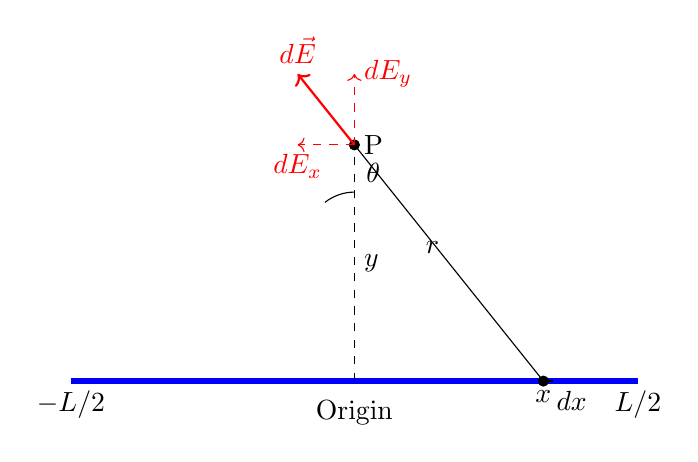
\begin{tikzpicture}[scale=1.2]
    % Draw the rod on the x-axis
    \draw[line width=2pt, blue] (-3,0) -- (3,0);
    \node[below] at (-3,0) {$-L/2$};
    \node[below] at (3,0) {$L/2$};
    \node[below] at (0,-0.1) {Origin};

    % Draw point P and relevant lines
    \filldraw (0,2.5) circle (1.5pt) node[right] {P};
    \draw[dashed] (0,0) -- (0,2.5) node[midway, right] {$y$};

    % Define a point dx on the rod
    \def\x{2}
    \filldraw (\x,0) circle (1.5pt) node[below] {$x$};
    \node[below] at (\x+0.3, 0) {$dx$};
    \draw[thick] (\x,0) -- (\x+0.1,0);

    % Lines and vectors from dx to P
    \draw (\x,0) -- (0,2.5) node[midway, above left] {$r$};
    \draw[->, red, thick] (0,2.5) -- (0-0.6, 2.5+0.75) node[above] {$d\vec{E}$};
    \draw[->, red, dashed] (0,2.5) -- (0, 2.5+0.75) node[right] {$dE_y$};
    \draw[->, red, dashed] (0,2.5) -- (0-0.6, 2.5) node[below] {$dE_x$};

    % Angle theta
    \draw (0, 2) arc (90:128.6:0.5);
    \node at (0.2, 2.2) {$\theta$};
\end{tikzpicture}
\end{center}

\subsubsection*{Explanation and Solution}
\paragraph{(a) Electric Field at Point P}
We use the principle of superposition. A small element of charge is $dq = \lambda dx$. The magnitude of the electric field $dE$ from this element is:
$$ dE = \frac{1}{4\pi\epsilon_0} \frac{dq}{r^2} = \frac{\lambda}{4\pi\epsilon_0} \frac{dx}{x^2 + y^2} $$
By symmetry, the horizontal components of the electric field cancel out. We only need to integrate the vertical components, $dE_y = dE \cos\theta$, where $\cos\theta = \frac{y}{\sqrt{x^2 + y^2}}$.
$$ dE_y = \frac{\lambda y}{4\pi\epsilon_0(x^2 + y^2)^{3/2}} dx $$
To find the total electric field $E$, we integrate from $x = -L/2$ to $x = L/2$:
$$ E = E_y = \int_{-L/2}^{L/2} \frac{\lambda y}{4\pi\epsilon_0(x^2 + y^2)^{3/2}} dx = \frac{\lambda}{4\pi\epsilon_0 y} \left[ \frac{x}{\sqrt{x^2+y^2}} \right]_{-L/2}^{L/2} = \frac{\lambda L}{2\pi\epsilon_0 y\sqrt{L^2 + 4y^2}} $$
The direction of the electric field is along the positive y-axis.
$$ \vec{E} = \frac{\lambda L}{2\pi\epsilon_0 y\sqrt{L^2 + 4y^2}} \hat{j} $$

\paragraph{(b) Limit for an Infinitely Long Rod}
We now consider the case where $L \to \infty$.
$$ E = \lim_{L\to\infty} \frac{\lambda L}{2\pi\epsilon_0 y\sqrt{L^2 + 4y^2}} = \lim_{L\to\infty} \frac{\lambda L}{2\pi\epsilon_0 yL\sqrt{1 + 4y^2/L^2}} = \frac{\lambda}{2\pi\epsilon_0 y} $$
This is the standard result for the electric field from an infinite line of charge.

\hrulefill

\subsection{Problem 2: The Charged Semicircle}
\subsubsection*{Problem Statement}
A thin, non-conducting rod is bent into the shape of a semicircle of radius $R$.
\begin{enumerate}
    \item[(a)] The rod is uniformly charged with a total positive charge $Q$. Find the magnitude and direction of the electric field at the center of the semicircle (point O).
    \item[(b)] What would be the electric field at point O if the charge distribution were non-uniform, given by $\lambda(\theta) = \lambda_0 \sin(\theta)$?
\end{enumerate}

\begin{center}
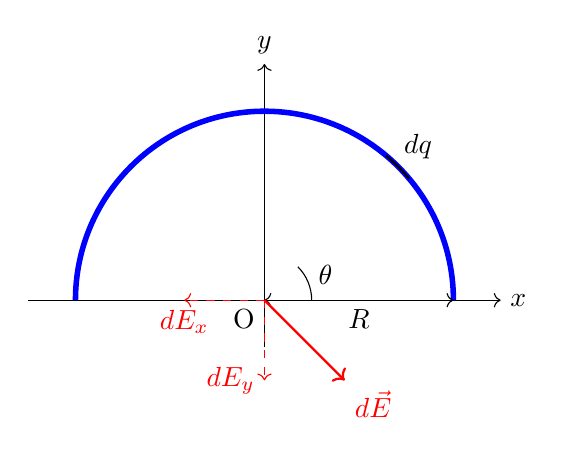
\begin{tikzpicture}[scale=1.2]
    % Axes
    \draw[->] (-2.5,0) -- (2.5,0) node[right] {$x$};
    \draw[->] (0,-0.5) -- (0,2.5) node[above] {$y$};
    \node[below left] at (0,0) {O};

    % Semicircle
    \draw[line width=2pt, blue] (180:2) arc (180:0:2);
    \draw[<->] (0,0) -- (0:2) node[midway, below] {$R$};

    % Charge element dq
    \def\angle{45}
    \draw[thick] (\angle-5:2) arc (\angle-5:\angle+5:2);
    \node at (\angle:2.3) {$dq$};
    
    % Field vector dE from dq
    \draw[->, red, thick] (0,0) -- (-\angle:1.2) node[below right] {$d\vec{E}$};
    \draw[->, red, dashed] (0,0) -- ({-cos(\angle)*1.2}, 0) node[below] {$dE_x$};
    \draw[->, red, dashed] (0,0) -- (0, {-sin(\angle)*1.2}) node[left] {$dE_y$};

    % Angle theta
    \draw (0.5,0) arc (0:\angle:0.5);
    \node at (\angle/2:0.7) {$\theta$};
\end{tikzpicture}
\end{center}

\subsubsection*{Explanation and Solution}
\paragraph{(a) Uniformly Charged Semicircle}
The uniform linear charge density is $\lambda = Q/(\pi R)$. The charge element is $dq = \lambda R \, d\theta$.
The electric field from this element is $dE = \frac{1}{4\pi\epsilon_0}\frac{dq}{R^2} = \frac{\lambda}{4\pi\epsilon_0 R} d\theta$.
By symmetry, the x-components cancel. We integrate the y-components, $dE_y = -dE \sin\theta$:
$$ E_y = \int_0^\pi -\frac{\lambda}{4\pi\epsilon_0 R} \sin\theta \, d\theta = -\frac{\lambda}{4\pi\epsilon_0 R} [-\cos\theta]_0^\pi = -\frac{2\lambda}{4\pi\epsilon_0 R} = -\frac{\lambda}{2\pi\epsilon_0 R} $$
Substituting $\lambda = Q/(\pi R)$:
$$ \vec{E} = -\frac{Q}{2\pi^2\epsilon_0 R^2} \hat{j} $$

\paragraph{(b) Non-uniformly Charged Semicircle}
With $\lambda(\theta) = \lambda_0 \sin\theta$, the charge element is $dq = \lambda_0 R \sin\theta \, d\theta$.
The x-component of the field integrates to zero. The y-component is:
$$ E_y = \int_0^\pi -\frac{1}{4\pi\epsilon_0 R^2} (\lambda_0 R \sin\theta \, d\theta) \sin\theta = -\frac{\lambda_0}{4\pi\epsilon_0 R} \int_0^\pi \sin^2\theta \, d\theta $$
$$ E_y = -\frac{\lambda_0}{4\pi\epsilon_0 R} \left[ \frac{\theta}{2} - \frac{\sin(2\theta)}{4} \right]_0^\pi = -\frac{\lambda_0}{4\pi\epsilon_0 R} \left( \frac{\pi}{2} \right) = -\frac{\lambda_0}{8\epsilon_0 R} $$
The total electric field is $\vec{E} = -\frac{\lambda_0}{8\epsilon_0 R} \hat{j}$.

\newpage
\section{Electric Potential Calculations}

\subsection{Problem 3: The Charged Ring}
\subsubsection*{Problem Statement}
A thin ring of radius $a$ carries a total charge $Q$ distributed uniformly.
\begin{enumerate}
    \item[(a)] Find the electric potential at a point P located a distance $x$ from the center of the ring along its axis of symmetry.
    \item[(b)] Using the result from part (a), find the electric field at point P.
    \item[(c)] What is the potential at the center of the ring? How does this relate to the electric field at the center?
\end{enumerate}

\begin{center}
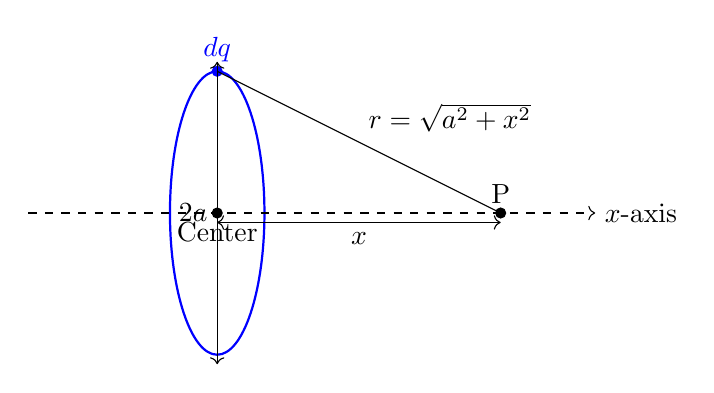
\begin{tikzpicture}[scale=1.2]
    % Ring in perspective
    \draw[blue, thick] (0,0) ellipse (0.5 and 1.5);
    \filldraw[blue] (0,1.5) circle (1.5pt) node[above] {$dq$};

    % Axis and points
    \draw[->, dashed] (-2,0) -- (4,0) node[right] {$x$-axis};
    \filldraw (0,0) circle (1.5pt) node[below] {Center};
    \filldraw (3,0) circle (1.5pt) node[above] {P};
    
    % Dimensions
    \draw[<->] (0,-1.6) -- (0,1.6) node[midway, left] {$2a$};
    \draw[<->] (0,-0.1) -- (3,-0.1) node[midway, below] {$x$};
    
    % Distance r
    \draw (0,1.5) -- (3,0) node[midway, above right] {$r = \sqrt{a^2+x^2}$};
\end{tikzpicture}
\end{center}

\subsubsection*{Explanation and Solution}
\paragraph{(a) Electric Potential at P}
Every point on the ring is equidistant from P, at $r = \sqrt{a^2 + x^2}$.
The potential $dV$ due to $dq$ is $dV = \frac{1}{4\pi\epsilon_0} \frac{dq}{r}$. To find the total potential $V$, we integrate over the ring.
$$ V = \int dV = \int \frac{1}{4\pi\epsilon_0} \frac{dq}{\sqrt{a^2 + x^2}} = \frac{1}{4\pi\epsilon_0\sqrt{a^2 + x^2}} \int dq $$
$$ V(x) = \frac{Q}{4\pi\epsilon_0\sqrt{a^2 + x^2}} $$

\paragraph{(b) Electric Field from Potential}
The electric field along the axis is $E_x = -\frac{dV}{dx}$.
$$ E_x = -\frac{d}{dx} \left( \frac{Q}{4\pi\epsilon_0}(a^2 + x^2)^{-1/2} \right) = -\frac{Q}{4\pi\epsilon_0} \left(-\frac{1}{2}(a^2 + x^2)^{-3/2}(2x)\right) $$
$$ E_x = \frac{Qx}{4\pi\epsilon_0(a^2 + x^2)^{3/2}} $$
The electric field vector is $\vec{E} = \frac{Qx}{4\pi\epsilon_0(a^2 + x^2)^{3/2}} \hat{i}$.

\paragraph{(c) Potential and Field at the Center}
At the center, $x=0$.
The potential is $V(0) = \frac{Q}{4\pi\epsilon_0 a}$, which is non-zero.
The electric field is $E_x(0) = 0$.

\hrulefill

\subsection{Problem 4: The Solid Sphere of Charge}
\subsubsection*{Problem Statement}
A solid insulating sphere of radius $R$ has a uniform volume charge density $\rho$. Find the electric potential for $r > R$ and $r < R$, assuming $V(\infty)=0$.

\begin{center}
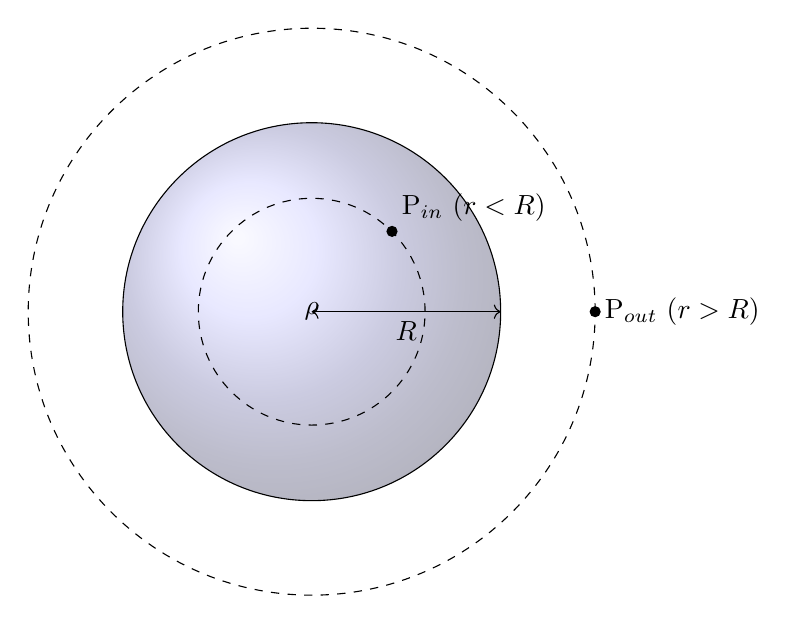
\begin{tikzpicture}[scale=1.2]
    % Sphere
    \shade[ball color=blue!30!white, opacity=0.4] (0,0) circle (2cm);
    \draw (0,0) circle (2cm);
    \node at (0,0) {$\rho$};
    \draw[<->] (0,0) -- (2,0) node[midway, below] {$R$};
    
    % Gaussian surfaces and points
    \draw[dashed] (0,0) circle (3cm); % r > R
    \filldraw (3,0) circle (1.5pt) node[right] {P$_{out}$ ($r>R$)};
    \draw[dashed] (0,0) circle (1.2cm); % r < R
    \filldraw (0.85, 0.85) circle (1.5pt) node[above right] {P$_{in}$ ($r<R$)};
\end{tikzpicture}
\end{center}

\subsubsection*{Explanation and Solution}
Using Gauss's Law, with total charge $Q = \rho \frac{4}{3}\pi R^3$:
\begin{itemize}
    \item \textbf{Outside ($r > R$):} $E_{out} = \frac{Q}{4\pi\epsilon_0 r^2}$.
    \item \textbf{Inside ($r < R$):} $E_{in} = \frac{Q r}{4\pi\epsilon_0 R^3}$.
\end{itemize}
\paragraph{(a) Potential Outside the Sphere ($r > R$)}
$$ V_{out}(r) = -\int_\infty^r \frac{Q}{4\pi\epsilon_0 (r')^2} \, dr' = \left[ \frac{Q}{4\pi\epsilon_0 r'} \right]_\infty^r = \frac{Q}{4\pi\epsilon_0 r} $$
\paragraph{(b) Potential Inside the Sphere ($r < R$)}
$$ V_{in}(r) = V(R) - \int_R^r E_{in} \, dr' = \frac{Q}{4\pi\epsilon_0 R} - \int_R^r \frac{Qr'}{4\pi\epsilon_0 R^3} \, dr' $$
$$ V_{in}(r) = \frac{Q}{4\pi\epsilon_0 R} - \frac{Q}{4\pi\epsilon_0 R^3} \left[ \frac{(r')^2}{2} \right]_R^r = \frac{Q}{4\pi\epsilon_0 R} - \frac{Q}{8\pi\epsilon_0 R^3}(r^2 - R^2) = \frac{Q(3R^2 - r^2)}{8\pi\epsilon_0 R^3} $$

\newpage
\section{Simple Harmonic Motion in Electrostatics}

\subsection{Problem 5: The Oscillating Dipole}
\subsubsection*{Problem Statement}
An electric dipole $\vec{p}$ is placed in a uniform electric field $\vec{E}$. If slightly displaced from its stable equilibrium, show that it undergoes simple harmonic motion.

\begin{center}
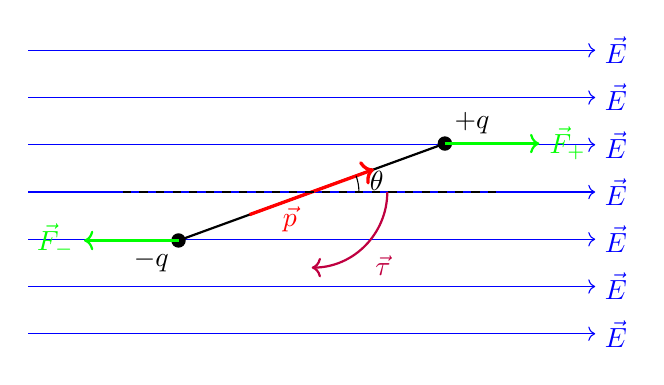
\begin{tikzpicture}[scale=1.2]
    % Uniform E-field
    \foreach \y in {-1.5, -1, -0.5, 0, 0.5, 1, 1.5}
    \draw[->, blue] (-3, \y) -- (3, \y) node[right] {$\vec{E}$};

    % Dipole
    \def\angle{20}
    \draw[thick] ({-1.5*cos(\angle)}, {-1.5*sin(\angle)}) -- ({1.5*cos(\angle)}, {1.5*sin(\angle)});
    \filldraw ({1.5*cos(\angle)}, {1.5*sin(\angle)}) circle (2pt) node[above right] {$+q$};
    \filldraw ({-1.5*cos(\angle)}, {-1.5*sin(\angle)}) circle (2pt) node[below left] {$-q$};
    \draw[->, very thick, red] ({-0.7*cos(\angle)}, {-0.7*sin(\angle)}) -- ({0.7*cos(\angle)}, {0.7*sin(\angle)}) node[midway, below left=2pt] {$\vec{p}$};
    
    % Forces
    \draw[->, green, thick] ({1.5*cos(\angle)}, {1.5*sin(\angle)}) -- ({1.5*cos(\angle)+1}, {1.5*sin(\angle)}) node[right] {$\vec{F}_+$};
    \draw[->, green, thick] ({-1.5*cos(\angle)}, {-1.5*sin(\angle)}) -- ({-1.5*cos(\angle)-1}, {-1.5*sin(\angle)}) node[left] {$\vec{F}_-$};

    % Angle and Torque
    \draw[dashed] (-2,0) -- (2,0);
    \draw (0.5,0) arc (0:\angle:0.5);
    \node at (\angle/2:0.7) {$\theta$};
    \draw[->, purple, thick] (0.8,0) arc (0:-90:0.8) node[midway, below right] {$\vec{\tau}$};
\end{tikzpicture}
\end{center}

\subsubsection*{Explanation and Solution}
The torque on the dipole is $\vec{\tau} = \vec{p} \times \vec{E}$, with magnitude $\tau = -pE\sin\theta$. For small angles, $\sin\theta \approx \theta$, so:
$$ \tau \approx -pE\theta $$
From Newton's second law for rotation, $\tau = I\alpha = I\frac{d^2\theta}{dt^2}$.
$$ I\frac{d^2\theta}{dt^2} = -pE\theta \implies \frac{d^2\theta}{dt^2} + \left(\frac{pE}{I}\right)\theta = 0 $$
This is the SHM equation, with angular frequency $\omega = \sqrt{\frac{pE}{I}}$.

\hrulefill

\subsection{Problem 6: The Charged Particle and the Ring}
\subsubsection*{Problem Statement}
A particle of mass $m$ and charge $-q$ is placed on the axis of a uniformly charged ring (charge $Q$, radius $R$) at a small distance $x$ from the center. Show it executes SHM.

\begin{center}
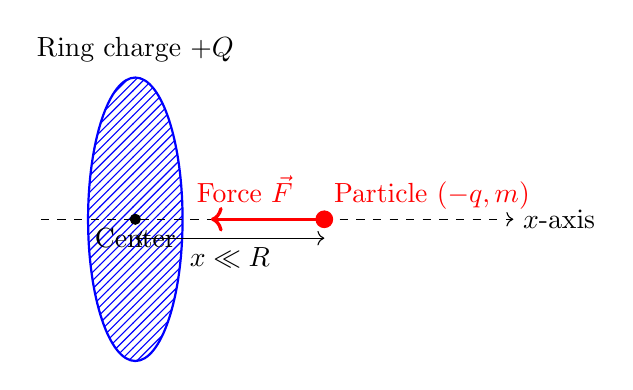
\begin{tikzpicture}[scale=1.2]
    % Ring in perspective
    \draw[blue, thick, pattern=north east lines, pattern color=blue] (0,0) ellipse (0.5 and 1.5);
    \node at (0, 1.8) {Ring charge $+Q$};
    
    % Axis and points
    \draw[->, dashed] (-1,0) -- (4,0) node[right] {$x$-axis};
    \filldraw (0,0) circle (1.5pt) node[below] {Center};
    
    % Particle and Force
    \filldraw[red] (2,0) circle (2.5pt) node[above right] {Particle ($-q, m$)};
    \draw[->, very thick, red] (2,0) -- (0.8,0) node[above=2pt, pos=0.7] {Force $\vec{F}$};
    
    % Dimensions
    \draw[<->] (0,-0.2) -- (2,-0.2) node[midway, below] {$x \ll R$};
\end{tikzpicture}
\end{center}

\subsubsection*{Explanation and Solution}
The electric field on the axis of the ring is $E_x = \frac{Qx}{4\pi\epsilon_0(R^2 + x^2)^{3/2}}$.
The force on the particle with charge $-q$ is:
$$ F_x = (-q)E_x = -\frac{Qqx}{4\pi\epsilon_0(R^2 + x^2)^{3/2}} $$
For small displacements, $x \ll R$, we have $R^2+x^2 \approx R^2$. The force becomes:
$$ F_x \approx -\left(\frac{Qq}{4\pi\epsilon_0 R^3}\right)x $$
This is a linear restoring force, $F_x = -Kx$, with $K = \frac{Qq}{4\pi\epsilon_0 R^3}$.
Using Newton's second law, $F = ma$:
$$ m\frac{d^2x}{dt^2} = -\left(\frac{Qq}{4\pi\epsilon_0 R^3}\right)x \implies \frac{d^2x}{dt^2} + \left(\frac{Qq}{4\pi\epsilon_0 mR^3}\right)x = 0 $$
This is the equation for SHM with $\omega^2 = \frac{Qq}{4\pi\epsilon_0 mR^3}$. The frequency is:
$$ f = \frac{\omega}{2\pi} = \frac{1}{2\pi}\sqrt{\frac{Qq}{4\pi\epsilon_0 mR^3}} $$

\newpage
\section{Additional Simple Harmonic Motion Problem}

\subsection{Problem 7: The Particle in the Tunnel}
\subsubsection*{Problem Statement}
A solid insulating sphere of radius $R$ has a total positive charge $+Q$ distributed uniformly throughout its volume. A narrow tunnel is drilled through the center of the sphere along one of its diameters. A small particle of mass $m$ and negative charge $-q$ is placed in the tunnel and released from rest at a distance $x$ ($x < R$) from the center.

\begin{enumerate}
    \item[(a)] Show that the particle experiences a linear restoring force and thus will execute simple harmonic motion.
    \item[(b)] Determine the frequency of this oscillation.
\end{enumerate}

\begin{center}
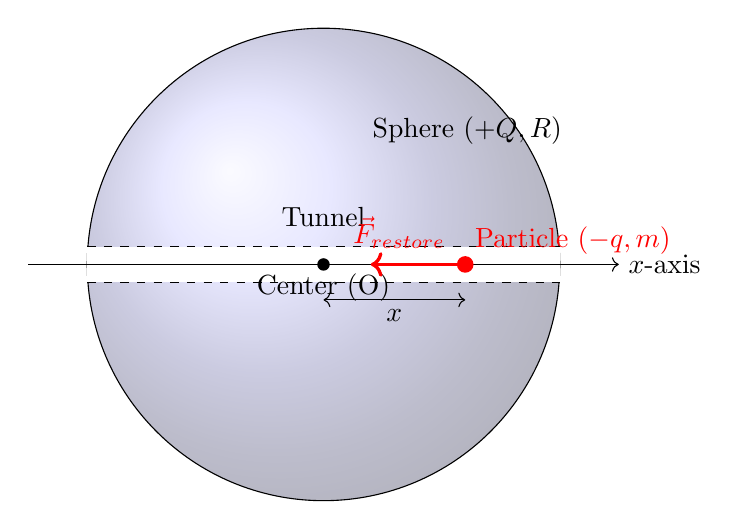
\begin{tikzpicture}[scale=1.5]
    % Draw the sphere with shading
    \shade[ball color=blue!30!white, opacity=0.4] (0,0) circle (2cm);
    \draw (0,0) circle (2cm) node[above right=1.4cm and 0.5cm] {Sphere ($+Q, R$)};

    % Draw the tunnel
    \fill[white] (-2,-0.15) rectangle (2,0.15);
    \draw[dashed] (-2, 0.15) -- (2, 0.15);
    \draw[dashed] (-2,-0.15) -- (2,-0.15);
    \node at (0, 0.4) {Tunnel};

    % Mark the center and the axes
    \fill (0,0) circle (1.5pt) node[below] {Center (O)};
    \draw[->, thin] (-2.5,0) -- (2.5,0) node[right] {$x$-axis};

    % Place the particle
    \def\xpos{1.2}
    \fill[red] (\xpos,0) circle (2pt) node[above right] {Particle ($-q, m$)};
    \draw[<->] (0, -0.3) -- (\xpos, -0.3) node[midway, below] {$x$};
    
    % Draw the restoring force vector
    \draw[->, red, very thick] (\xpos,0) -- (\xpos-0.8, 0) node[above=2pt, pos=0.7] {$\vec{F}_{restore}$};
\end{tikzpicture}
\end{center}

\subsection*{Explanation and Solution}
\paragraph{(a) Proving Simple Harmonic Motion}
For the particle to execute simple harmonic motion (SHM), it must be subjected to a restoring force that is directly proportional to its displacement from an equilibrium position. In this case, the equilibrium position is the center of the sphere ($x=0$), where the net force is zero by symmetry. The force has the form $F = -Kx$, where $K$ is a positive constant.

\begin{enumerate}
    \item \textbf{Find the Electric Field Inside the Sphere:} We use Gauss's Law to find the electric field $\vec{E}$ at a distance $x$ from the center (where $x < R$). We consider a spherical Gaussian surface of radius $x$. The charge enclosed, $Q_{enc}$, is proportional to the volume:
    $$ Q_{enc} = Q \left( \frac{\text{Volume of radius } x}{\text{Total Volume}} \right) = Q \frac{\frac{4}{3}\pi x^3}{\frac{4}{3}\pi R^3} = Q \frac{x^3}{R^3} $$
    Applying Gauss's Law, $\oint \vec{E} \cdot d\vec{A} = \frac{Q_{enc}}{\epsilon_0}$:
    $$ E (4\pi x^2) = \frac{1}{\epsilon_0} \left( Q \frac{x^3}{R^3} \right) $$
    Solving for the magnitude of the electric field $E$:
    $$ E = \frac{Qx}{4\pi\epsilon_0 R^3} $$
    The electric field is directed radially outward and its magnitude is proportional to the distance $x$ from the center.

    \item \textbf{Calculate the Force on the Particle:} The electric force $\vec{F}$ on the particle with charge $-q$ is given by $\vec{F} = (-q)\vec{E}$. Since the particle is constrained to the tunnel (the x-axis), we consider the force along this axis:
    $$ F_x = (-q) E_x = -q \left( \frac{Qx}{4\pi\epsilon_0 R^3} \right) $$
    $$ F_x = -\left( \frac{Qq}{4\pi\epsilon_0 R^3} \right) x $$
    
    \item \textbf{Conclusion:} The force $F_x$ is directly proportional to the displacement $x$ and the negative sign indicates it is a restoring force (it always points opposite to the displacement vector, towards the center). This is precisely the condition for simple harmonic motion.
\end{enumerate}

\paragraph{(b) Determining the Frequency}
We can compare our force equation to Hooke's Law, $F = -Kx$. By comparison, the effective "spring constant" $K$ is:
$$ K = \frac{Qq}{4\pi\epsilon_0 R^3} $$
The angular frequency $\omega$ for a mass-spring system is given by $\omega = \sqrt{K/m}$.
$$ \omega = \sqrt{\frac{Qq}{4\pi\epsilon_0 m R^3}} $$
The linear frequency $f$ is related to the angular frequency by $\omega = 2\pi f$. Therefore, the frequency of the oscillation is:
$$ f = \frac{\omega}{2\pi} = \frac{1}{2\pi} \sqrt{\frac{Qq}{4\pi\epsilon_0 m R^3}} $$

\end{document}